\documentclass{beamer}

\usepackage[brazil]{babel}
\usepackage[utf8]{inputenc}
\usepackage[T1]{fontenc}
\usepackage{listings}

\usepackage{adjustbox}

\usetheme{Madrid}
\setbeamertemplate{navigation symbols}{}

\lstset{
language=sql,
basicstyle=\ttfamily\tiny,
backgroundcolor=\color{white},
keywordstyle=\color{blue}\bfseries,
stringstyle=\color{red},
commentstyle=\color{green},
%morecomment=[s][\color{green}]{/**}{*/},
showspaces=false,
showstringspaces=false,
morekeywords={database,modify,references,delimiter,procedure,begin,function,return,returns,if,elseif,after,for,each,row},
literate=
{á}{{\'a}}1
{Á}{{\'A}}1
{à}{{\`a}}1 
{À}{{\`A}}1
{â}{{\^a}}1 
{Â}{{\^A}}1
{ã}{{\~a}}1
{Ã}{{\~A}}1
{ä}{{\"a}}1
{Ä}{{\"A}}1
{é}{{\'e}}1
{É}{{\'E}}1
{è}{{\`e}}1
{È}{{\`E}}1
{ê}{{\^e}}1
{Ê}{{\^E}}1
{ẽ}{{\~e}}1
{Ẽ}{{\~E}}1 
{ë}{{\"e}}1
{Ë}{{\"E}}1
{í}{{\'i}}1
{Í}{{\'I}}1
{ì}{{\`i}}1
{Ì}{{\`I}}1
{î}{{\^i}}1
{Î}{{\^I}}1
{ĩ}{{\~i}}1
{Ĩ}{{\~I}}1
{ï}{{\"i}}1
{Ï}{{\"I}}1
{ó}{{\'o}}1
{Ó}{{\'O}}1
{ò}{{\`o}}1
{Ò}{{\`O}}1
{ô}{{\^o}}1
{Ô}{{\^O}}1
{õ}{{\~o}}1
{Õ}{{\~O}}1
{ö}{{\"o}}1
{Ö}{{\"O}}1
{ú}{{\'u}}1
{Ú}{{\'U}}1
{ù}{{\`u}}1
{Ù}{{\`U}}1
{û}{{\^u}}1
{Û}{{\^U}}1
{ũ}{{\~u}}1
{Ũ}{{\~U}}1
{ü}{{\"u}}1
{Ü}{{\"U}}1
{ç}{{\c{c}}}1
{Ç}{{\c{C}}}1
}

\title[Banco de Dados]{Banco de Dados}

\author[Diego S. C. Nascimento]{Diego Silveira Costa Nascimento}

\institute[IFRN]{
Instituto Federal de Educação, Ciência e Tecnologia do Rio Grande do Norte\\
diego.nascimento@ifrn.edu.br
}

\date[\today]{\today}

\begin{document}

\begin{frame}[plain]
	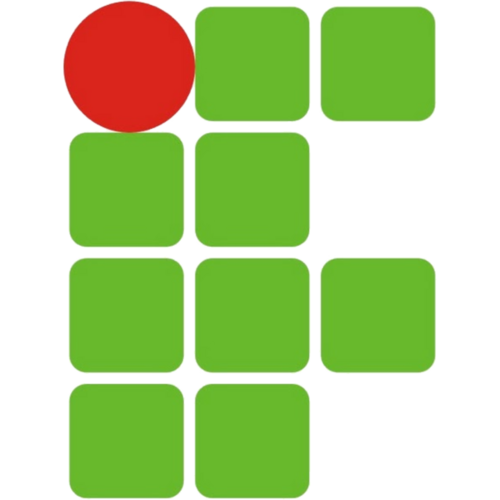
\includegraphics[scale=0.2]{IFRN}
	\titlepage
\end{frame}

\logo{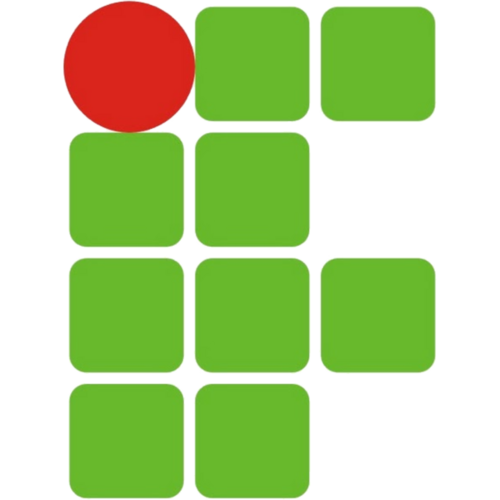
\includegraphics[scale=0.1]{IFRN}}

\begin{frame}
	\frametitle{Ementa}
  	\tableofcontents
\end{frame}

\AtBeginSection[]{
	\begin{frame}
		\frametitle{Ementa}
		\tableofcontents[currentsection]
	\end{frame}
}

\section{Introdução}

\begin{frame}
\frametitle{Banco de Dados}

\begin{block}{Definição}
	São conjuntos de registros dispostos em estrutura regular que possibilita a
	organização dos dados e produção de informação.
\end{block}
\end{frame}

\begin{frame}
\frametitle{Sistema Gerenciador de Banco de Dados (SGBD)}

\begin{block}{Definição}
É uma coleção de programas de propósito geral que facilita os processos de
definição, construção, manipulação e compartilhamento de bancos entre
vários usuários e aplicações.
\end{block}
\end{frame}

\section{Abordagem Entidade-relacionamento}

\begin{frame}
\frametitle{Modelo de 	Banco de Dados}

\begin{block}{Definição}
	É uma descrição dos tipos de informações que estão armazenadas em um
	banco de dados.
\end{block} \vfill

\begin{itemize}
	\item Para construir um modelo de dados usa-se uma linguagem de
	modelagem de dados;
	\item A linguagem de modelagem pode ser textual ou gráfica;
	\item Existem linguagens de modelagem para descrever modelos de dados
	em diferentes níveis de abstração e objetivos; e
	\item Cada representação de um modelo de dados recebe a denominação de
	esquema de banco de dados.
\end{itemize}
\end{frame}

\begin{frame}
\frametitle{Entidade}

\begin{block}{Definição}
	Conjunto de objetos da realidade modelada sobre os quais deseja-se manter
	informações o banco de dados.
\end{block} 
\end{frame}

\begin{frame}
\frametitle{Atributo}

\begin{block}{Definição}
	Dado que é associado a cada ocorrêcia de uma entidade.
\end{block} 
\end{frame}

\begin{frame}
\frametitle{Identificador da Entidade}

\begin{block}{Definição}
	Um identificador é um conjunto de um ou mais atributos (e possivelmente
	relacionamentos, como visto abaixo) cujos valores servem para distinguir
	uma ocorrência da entidade das demais ocorrências da mesma entidade.
\end{block} \vfill

A identificação pode ser:
\begin{itemize}
	\item Simples; ou
	\item Composta.
\end{itemize}
\end{frame}

\begin{frame}
\frametitle{Relacionamento}

\begin{block}{Definição}
	Conjunto de associações entre ocorrência de entidades.
\end{block}
\end{frame}

\begin{frame}
\frametitle{Cardinalidade de Relacionamento}

\begin{block}{Definição}
É o número (mínimo, máximo) de ocorrências de entidade associadas a
uma ocorrência da entidade em questão através do relacionamento.
\end{block} \vfill

	Classificação de relacionamentos binários:
	\begin{itemize}
	\item 1:1 (um-para-um);
	\item 1:N (um-para-muitos);
	\item N:N (muitos-para-muitos);
	\end{itemize}
\end{frame}

\section{Abordagem Relacional}

\begin{frame}
\frametitle{Tabela}

\begin{itemize}
	\item É um conjunto não ordenado de linhas (tuplas);
	\item Cada linha é composta por uma série de campos (valor do atributo);
	\item Cada campo é identificado por nome de campo (nome de atributo); e
	\item O conjunto de campos das linhas de uma tabela que possuem o
	mesmo nome formam uma coluna.
\end{itemize}
\end{frame}

\begin{frame}
\frametitle{Chave}

\begin{block}{Definição}
	E a forma na qual se estabelece relações entre linhas de tabelas de um
	banco de dados relacional.
\end{block}\vfill

Tipos de chave:
\begin{itemize}
	\item Primária; e 
	\item Estrangeira.
\end{itemize}
\end{frame}

\begin{frame}
\frametitle{Chave Primária}

\begin{block}{Definição}
	É uma coluna ou uma combinação de colunas cujos valores distinguem uma linha das demais dentro de uma tabela.
\end{block}\vfill

\begin{exampleblock}{Departamento}
\centering
\begin{tabular}{|c|l|}
		\hline
		CODIGO & DESCRICAO \\ \hline
		D1 & Compras \\ \hline
		D2 & Engenharia \\ \hline
		D3 & Vendas \\ \hline
\end{tabular}
\end{exampleblock}		
\end{frame}

\begin{frame}
\frametitle{Chave Estrangeira}

\begin{block}{Definição}
  É uma coluna cujos valores aparecem necessariamente na chave primária de uma tabela.
\end{block}\vfill

\begin{exampleblock}{Empregado}
\centering
\begin{tabular}{|c|l|c|}
	\hline
	CODIGO & NOME & COD\_DEPART  \\ \hline
	E1 & Souza & D1  \\ \hline
	E2 & Santos & D2 \\ \hline
	E3 & Silva &  D2\\ \hline
	E4 & Soares & D3 \\ \hline
\end{tabular}
\end{exampleblock}		
\end{frame}

\section{Normalização}

\begin{frame}
\frametitle{Normalização}

\begin{block}{Definição}
	É uma regra que deve ser obedecida por uma tabela para que esta seja
	considerada ``bem projetada''.
\end{block} \vfill

Tipos de normalização:
\begin{itemize}
	\item Primeira forma normal (1FN);
	\item Segunda forma normal (2FN);
	\item Terceira forma normal (3FN); e
	\item Quarta forma normal (4FN).
\end{itemize}

\end{frame}

\begin{frame}
\frametitle{Tabela Não Normalizada}

\begin{exampleblock}{Projeto\_Empregado}
\resizebox{\textwidth}{!}{
\begin{tabular}{| l | l | c | l | c | r | l | c | }
\hline	
COD\_PROJ & TIPO DESC & COD\_EMP & NOME & CAT & SAL & INI & DURAC \\\hline
LSC001 & Desenvolvimento Sistema de Estoque &  2146 & João & A1 & 4 & 01/11/91 & 24 \\\hline
LSC001 & Desenvolvimento Sistema de Estoque & 3145 & Sílvio & A2 & 4 & 02/10/91 & 24 \\\hline
LSC001 & Desenvolvimento Sistema de Estoque & 6126 & José & B1 & 9 & 03/10/92 & 18 \\\hline
LSC001 & Desenvolvimento Sistema de Estoque & 1214 & Carlos & A2 & 4 & 04/10/92 & 18 \\\hline
LSC001 & Desenvolvimento Sistema de Estoque & 8191 & Mário & A1 & 4 &01/11/92 & 12 \\\hline
PAG02 & Manutenção Sistema de RH & 8191 & Mário & A1 & 4 & 01/05/93 & 12 \\\hline
PAG02 & Manutenção Sistema de RH & 4112 & João & A2 & 4 & 04/01/91 & 24 \\\hline
PAG02 & Manutenção Sistema de RH & 6126 &José & B1 & 9 & 01/11/92& 12 \\\hline
\end{tabular}
}
\end{exampleblock}
\end{frame}

\begin{frame}
\frametitle{Primeira Forma Normal (1FN)}

\begin{block}{Definição}
	Diz-se que uma tabela está na primeira forma normal, quando ela não contém tabelas aninhadas.
\end{block}	
\end{frame}

\begin{frame}
\frametitle{Tabela na 1FN}

\begin{exampleblock}{Projeto}
\centering
\begin{tabular}{| l | l | l |}
\hline
COD & TIPO & DESC \\\hline
LSC001 & Desenvolvimento & Sistema de Estoque \\\hline
PAG02 & Manutenção & Sistema de RH \\\hline
\end{tabular}
\end{exampleblock}	\vfill

\begin{exampleblock}{Empregado}
\resizebox{\textwidth}{!}{
\begin{tabular}{| l | c |  l | c | r | l | c |}
	\hline
	COD\_PROJ & COD\_EMP & NOME & CAT & SAL & INI & DURAC \\\hline
	LSC001 & 2146 & João & A1 & 4 & 01/11/91 & 24 \\\hline
	LSC001 & 3145 & Sílvio & A2 & 4 & 02/10/91 & 24 \\\hline
	LSC001 & 6126 & José & B1 & 9 & 03/10/92 & 18 \\\hline
	LSC001 & 1214 & Carlos & A2 & 4 & 04/10/92 & 18 \\\hline
	LSC001  & 8191 & Mário & A1 & 4 & 01/11/92 & 12 \\\hline
	PAG02 & 8191 & Mário & A1 & 4 & 01/05/93 & 12 \\\hline
	PAG02 & 4112 & João & A2 & 4 & 04/01/91 & 24 \\\hline
	PAG02 & 6126 & José & B1 & 9 & 01/11/92 & 12 \\\hline
\end{tabular}
}
\end{exampleblock}	
\end{frame}

\begin{frame}
\frametitle{Dependência Funcional}

\begin{block}{Definição}
	Diz-se que uma coluna C2 depende funcionalmente de uma coluna C1 (ou
	que a coluna C1 determina a coluna C2) quando, em todas linhas da tabela,
	para cada valor de C1 que aparece na tabela, aparece o mesmo valor de C2.
\end{block}\vfill

\begin{exampleblock}{Exemplo}
\centering
\begin{tabular}{| c | r |}
	\hline
	CODIGO & SALARIO  \\\hline
 E1 & 10 \\\hline
 E3 & 10\\\hline
 E1 & 10 \\\hline
 E2 & 5 \\\hline
 E3 & 10\\\hline
 E2 & 5 \\\hline
 E1 & 10\\\hline
\end{tabular}
\end{exampleblock}
\end{frame}

\begin{frame}
\frametitle{Segunda Forma Normal (2FN)}

\begin{block}{Definição}
	Uma tabela encontra-se na segunda forma normal, quando, além de estar na 1FN, não contém dependências parciais.
\end{block}	
\end{frame}

\begin{frame}
\frametitle{Tabela na 2FN}

\begin{exampleblock}{Projeto\_Empregado}
	\centering
	\begin{tabular}{| l | c | l | c |}
		\hline
		COD\_PROJ & COD\_EMP &  INI & DURAC \\\hline
		LSC001 & 2146 & 01/11/91 & 24 \\\hline
		LSC001 & 3145 & 02/10/91 & 24 \\\hline
		LSC001 & 6126 & 03/10/92 & 18 \\\hline
		LSC001 & 1214 & 04/10/92 & 18 \\\hline
		LSC001  & 8191 &01/11/92 & 12 \\\hline
		PAG02 & 8191 & 01/05/93 & 12 \\\hline
		PAG02 & 4112 & 04/01/91 & 24 \\\hline
		PAG02 & 6126 &01/11/92 & 12 \\\hline
	\end{tabular}
\end{exampleblock}	
\end{frame}

\begin{frame}
\frametitle{Tabela na 2FN}

\begin{exampleblock}{Empregado}
\centering
\begin{tabular}{| c | l | c | r | }
	\hline
	COD\_EMP & NOME & CAT & SAL \\\hline
	2146 & João & A1 & 4 \\\hline
	3145 & Sílvio & A2 & 4 \\\hline
	6126 & José & B1 & 9 \\\hline
	1214 & Carlos & A2 & 4  \\\hline
	8191 & Mário & A1 & 4  \\\hline
	8191 & Mário & A1 & 4  \\\hline
	4112 & João & A2 & 4  \\\hline
	6126 & José & B1 & 9  \\\hline
\end{tabular}
\end{exampleblock}	
\end{frame}

\begin{frame}
\frametitle{Terceira Forma Normal (3FN)}

\begin{block}{Definição}
	Uma tabela encontra-se na terceira forma normal, quando, além de estar na 2FN, não contém dependências transitivas.
\end{block}	
\end{frame}

\begin{frame}
\frametitle{Tabela na 3FN}

\begin{exampleblock}{Empregado}
	\centering
	\begin{tabular}{| c | l | c | }
		\hline
		COD\_EMP & NOME & CAT \\\hline
		2146 & João & A1  \\\hline
		3145 & Sílvio & A2 \\\hline
		6126 & José & B1 \\\hline
		1214 & Carlos & A2 \\\hline
		8191 & Mário & A1 \\\hline
		8191 & Mário & A1 \\\hline
		4112 & João & A2 \\\hline
		6126 & José & B1 \\\hline
	\end{tabular}
\end{exampleblock}
\end{frame}

\begin{frame}
\frametitle{Tabela na 3FN}

\begin{exampleblock}{Categoria}
	\centering
	\begin{tabular}{| c | r | }
		\hline
		CAT & SAL \\\hline
		A1 & 4 \\\hline
		A2 & 4 \\\hline
		B1 & 9 \\\hline
	\end{tabular}
\end{exampleblock}	
\end{frame}

\begin{frame}
\frametitle{Quarta Forma Normal (4FN)}

\begin{block}{Definição}
Uma tabela encontra-se na quarta forma normal, quando, além de estar na 3FN, não contém dependências multi-valoradas.
\end{block}
\end{frame}

\begin{frame}
\frametitle{Incluindo Nova Entidade}

\begin{exampleblock}{Equipamento}
	\centering
	\begin{tabular}{| c | l | }
		\hline
		COD & DESC \\\hline
		EQ1 & Projetor \\\hline
		EQ2 & Notebook \\\hline
		EQ3 & Roteador \\\hline
	\end{tabular}
\end{exampleblock}	
\end{frame}

\begin{frame}
\frametitle{Incluindo Nova Entidade}

\begin{exampleblock}{Projeto\_Empregado\_Equipamento}
	\centering
	\begin{tabular}{| c | c | c | }
		\hline
COD\_PROJ & COD\_EMP & COD\_EQUI \\\hline
PAG02 & 8191 & EQ1 \\\hline
PAG02 & 4112 & EQ1 \\\hline
PAG02 & 6126 & EQ1 \\\hline
PAG02 & 8191 & EQ2 \\\hline
PAG02 & 4112 & EQ2 \\\hline
PAG02 & 6126 & EQ2 \\\hline
PAG02 & 8191 & EQ3 \\\hline
PAG02 & 4112 & EQ3 \\\hline
PAG02 & 6126 & EQ3 \\\hline
\end{tabular}
\end{exampleblock}	
\end{frame}

\begin{frame}
\frametitle{Tabela na 4FN}

\begin{exampleblock}{Projeto\_Equipamento}
	\centering
	\begin{tabular}{| c | r |}
		\hline
COD\_PROJ & COD\_EQUI \\\hline
PAG02 & E1 \\\hline
PAG02 & E2 \\\hline
PAG02 & E3 \\\hline
	\end{tabular}
\end{exampleblock}
\end{frame}

\section{Structured Query Language (SQL)}

\begin{frame}
\frametitle{Linguagem SQL}

\begin{itemize}
	\item É uma linguagem de pesquisa declarativa padrão para banco de dados relacional ;
	\item Implementada no projeto de pesquisa do System R da IBM em
	meados dos anos 70;
	\item Padronizada em 1986 e melhorada em 1989;
	\item SQL-2 ou SQL-92: Padrão hoje em vigor; e
	\item SQL-3: Em fase de desenvolvimento. Vai estender o padrão atual com
	conceitos de orientação a objeto e outros novos conceitos de BDs.
\end{itemize}
\end{frame}

\begin{frame}
\frametitle{Comandos SQL}

\begin{itemize}
	\item Definição de dados; e
	\item Manipulação dos dados.
\end{itemize}
\end{frame}

\begin{frame}
\frametitle{Comandos de Definição de Dados}

\begin{itemize}
	\item Criação e exclusão de banco de dados;
	\item Criação, alteração e exclusão de tabela;
	\begin{itemize}
		\item Especificação de restrições;
	\end{itemize}
	\item Criação de visão;
	\item Criação de procedimento armazenado;
	\item Criação de função; e
	\item Criação de gatilho.
\end{itemize}
\end{frame}

\begin{frame}[fragile]
\frametitle{Criando Banco de Dados}

\begin{block}{Estrutura}
\begin{lstlisting}
CREATE DATABASE <nome do banco>;
\end{lstlisting}
\end{block}\vfill

\begin{exampleblock}{Exemplo}
\begin{lstlisting}
CREATE DATABASE academico;
\end{lstlisting}
\end{exampleblock}
\end{frame}

\begin{frame}[fragile]
\frametitle{Criando Tabela}

\begin{block}{Estrutura}
\begin{lstlisting}
CREATE TABLE <nome da tabela>(
   <nome do atributo 1> <tipo de dado>,
   <nome do atributo 2> <tipo de dado>
)
\end{lstlisting}
\end{block}\vfill

\begin{exampleblock}{Exemplo}
\begin{lstlisting}
CREATE TABLE tb_aluno(
   matricula INT,
   nome VARCHAR(50),
   sexo CHAR
)
\end{lstlisting}
\end{exampleblock}
\end{frame}

\begin{frame}[fragile]
\frametitle{Criando Tabela}

\begin{exampleblock}{Exemplo}
\begin{lstlisting}
CREATE TABLE tb_disciplina(
   identificador INT,
   descricao VARCHAR(50),
   credito INT
)	
\end{lstlisting}\vfill

\begin{lstlisting}
CREATE TABLE tb_disciplina_cursada(
   matricula_aluno INT,
   identificador_disciplina INT,
   semestre INT,
   ano INT,
   nota FLOAT
)	
\end{lstlisting}
\end{exampleblock}
\end{frame}

\begin{frame}[fragile]
\frametitle{Alterando Tabela}

\begin{block}{Estrutura}
\begin{lstlisting}
ALTER TABLE <nome da tabela> 
ADD <nome do atributo> <tipo de dado>
\end{lstlisting}
\end{block}\vfill

\begin{exampleblock}{Exemplo}
\begin{lstlisting}
ALTER TABLE tb_aluno
ADD cpf VARCHAR(11)
\end{lstlisting}
\end{exampleblock}
\end{frame}

\begin{frame}
\frametitle{Comandos de Manipulação de Dados}

\begin{itemize}
	\item Inserir registros em tabelas;
	\item Selecionando registros;
	\item Atualizar registros em tabelas; e
	\item Excluir registros em tabelas.
\end{itemize}
\end{frame}

\begin{frame}[fragile]
\frametitle{Inserindo Valores}

\begin{block}{Estrutura}
\begin{lstlisting}
INSERT INTO <nome da tabela>
(<nome do atributo 1>,<nome do atributo 2>)
VALUES
('valor 1','valor 2')
\end{lstlisting}
\end{block}\vfill

\begin{exampleblock}{Exemplo}
\begin{lstlisting}
INSERT INTO tb_aluno
(matricula,nome,sexo,cpf)
VALUES
('1','João da Silva','M','12345678')
\end{lstlisting}
\end{exampleblock}
\end{frame}

\begin{frame}[fragile]
\frametitle{Selecionando Registros}

\begin{block}{Estrutura}
\begin{lstlisting}
SELECT <nome do atributo 1>, <nome do atributo 2>
FROM <nome da tabela>
\end{lstlisting}
\end{block}\vfill

\begin{exampleblock}{Exemplo}
\begin{lstlisting}
SELECT matricula, nome
FROM tb_aluno
\end{lstlisting}
\end{exampleblock}\vfill

\alert{Caso necessite selecionar todos os atributos de uma única vez, deve-se
	apenas utilizar o síbolo de asterisco (*) em substituição do(s) nome(s)
	da(s) coluna(s).}
\end{frame}

\begin{frame}[fragile]
\frametitle{Cláusula WHERE}

\begin{block}{Estrutura}
\begin{lstlisting}
SELECT <nome do atributo 1>, <nome do atributo 2>
FROM <nome da tabela>
WHERE <condição>
\end{lstlisting}
\end{block}\vfill

\begin{exampleblock}{Exemplo}
\begin{lstlisting}
SELECT matricula, nome
FROM tb_aluno
WHERE matricula = '1'
\end{lstlisting}
\end{exampleblock}
\end{frame}

\begin{frame}
\frametitle{Conectores Relacionais}

\begin{itemize}
	\item igual: =;
	\item maior: >;
	\item menor: <;
	\item maior igual: >=;
	\item menor igual: <=;
	\item diferente: <>;
	\item entre: between; e
	\item parte: like (Permitido o uso de máscara com \% entre aspas simples).
\end{itemize}
\end{frame}

\begin{frame}
\frametitle{Conectores Lógicos}

\begin{itemize}
	\item e: and;
	\item ou: or;
	\item é nulo: is null; e
	\item não é nulo: is not null.
\end{itemize}
\end{frame}

\begin{frame}[fragile]
\frametitle{Atualizando Valores}

\begin{block}{Estrutura}
\begin{lstlisting}
UPDATE <nome da tabela>
SET <nome do atributo> = '<valor>'
WHERE <condição>
\end{lstlisting}
\end{block}\vfill

\begin{exampleblock}{Exemplo}
\begin{lstlisting}
UPDATE tb_aluno
SET nome = 'João da Silva Filho'
WHERE matricula = '1'
\end{lstlisting}
\end{exampleblock}
\end{frame}

\begin{frame}[fragile]
\frametitle{Excluindo  Valores}

\begin{block}{Estrutura}
\begin{lstlisting}
DELETE FROM <nome da tabela>
WHERE <condição>
\end{lstlisting}
\end{block}\vfill

\begin{exampleblock}{Exemplo}
\begin{lstlisting}
DELETE FROM tb_aluno
WHERE matricula = '1'
\end{lstlisting}
\end{exampleblock}
\end{frame}

\begin{frame}
\frametitle{Especificando Restrições de Integridade}

\begin{itemize}
	\item Declarativas:
	\begin{itemize}
		\item Domínio;
		\item Vazio;
		\item Padrão;
		\item Checagem;
		\item Unicidade;
		\item Chave primária; e
		\item Referencial.
	\end{itemize}
	\item Procedimental:
	\begin{itemize}
	\item Procedimento armazenado
	\item Função; e
	\item Gatilho.
	\end{itemize}
\end{itemize}
\end{frame}

\begin{frame}[fragile]
\frametitle{Restrição de Vazio}

\begin{exampleblock}{Exemplo}
\begin{lstlisting}
ALTER TABLE tb_aluno
MODIFY COLUMN nome VARCHAR(30) NOT NULL;
\end{lstlisting}
\end{exampleblock}
\end{frame}

\begin{frame}[fragile]
\frametitle{Restrição de Padrão}

\begin{exampleblock}{Exemplo}
\begin{lstlisting}
ALTER TABLE tb_aluno
ALTER sexo SET DEFAULT 'M';
\end{lstlisting}
\end{exampleblock}
\end{frame}

\begin{frame}[fragile]
\frametitle{Restrição de Checagem}

\begin{exampleblock}{Exemplo}
\begin{lstlisting}
ALTER TABLE tb_disciplina_cursada
ADD CONSTRAINT ck_nota 
CHECK (nota>=0 AND nota<=10);
\end{lstlisting}
\end{exampleblock}
\end{frame}

\begin{frame}[fragile]
\frametitle{Restrição de Unicidade}

\begin{exampleblock}{Exemplo}
	\begin{lstlisting}
ALTER TABLE tb_aluno
ADD CONSTRAINT uc_cpf
UNIQUE (cpf);
	\end{lstlisting}
\end{exampleblock}
\end{frame}

\begin{frame}[fragile]
\frametitle{Restrição de Chave}

\begin{exampleblock}{Exemplos}
	\begin{lstlisting}
ALTER TABLE tb_aluno
ADD CONSTRAINT pk_aluno 
PRIMARY KEY (matricula);
	\end{lstlisting}

	\begin{lstlisting}
ALTER TABLE tb_disciplina
ADD CONSTRAINT pk_disciplina 
PRIMARY KEY (identificador);
	\end{lstlisting}
	
	\begin{lstlisting}
ALTER TABLE tb_disciplina_cursada
ADD CONSTRAINT pk_tb_disciplina_cursada
PRIMARY KEY (matricula_aluno,identificador_disciplina,semestre,ano)	
	\end{lstlisting}
\end{exampleblock}
\end{frame}

\begin{frame}[fragile]
\frametitle{Restrição de Referencial}

\begin{exampleblock}{Exemplos}
	\begin{lstlisting}
ALTER TABLE tb_disciplina_cursada
ADD CONSTRAINT fk_aluno
FOREIGN KEY (matricula_aluno)
REFERENCES tb_aluno(matricula);
	\end{lstlisting}
	
	\begin{lstlisting}
ALTER TABLE tb_disciplina_cursada
ADD CONSTRAINT fk_disciplina
FOREIGN KEY (identificador_disciplina)
REFERENCES tb_disciplina(identificador);
	\end{lstlisting}	
\end{exampleblock}
\end{frame}

\begin{frame}[fragile]
\frametitle{Visão}

\begin{block}{Estrutura}
	\begin{lstlisting}
CREATE VIEW <nome> AS
<consulta sql>;
	\end{lstlisting}
\end{block}\vfill

\begin{exampleblock}{Exemplo}
	\begin{lstlisting}
CREATE VIEW vw_aluno AS
SELECT nome, cpf
FROM vw_aluno;
	\end{lstlisting}
\end{exampleblock}
\end{frame}

\begin{frame}[fragile]
\frametitle{Procedimento Armazenado}

\begin{block}{Estrutura}
	\begin{lstlisting}
DELIMITER $

CREATE PROCEDURE <nome>(<parâmetro> <tipo do parâmetro>)
BEGIN
    <comando sql>;
END
$
	\end{lstlisting}
\end{block}\vfill

\begin{exampleblock}{Exemplo}
	\begin{lstlisting}
DELIMITER $

CREATE PROCEDURE inserir_aluno(a VARCHAR(30), b CHAR(1), c VARCHAR(11))
BEGIN
    INSERT INTO tb_aluno (nome, sexo,cpf) VALUES (a,b,c);
END
$	\end{lstlisting}
\end{exampleblock}
\end{frame}

\begin{frame}[fragile]
\frametitle{Função}

\begin{block}{Estrutura}
	\begin{lstlisting}
DELIMITER $

CREATE FUNCTION <nome>(<parâmetro> <tipo do parâmentro>) 
RETURNS <retorno do parâmentro>

BEGIN
    <código>;
END
$
	\end{lstlisting}
\end{block}
\end{frame}

\begin{frame}[fragile]
\frametitle{Função}

\begin{exampleblock}{Exemplo}
	\begin{lstlisting}
DELIMITER $
	
CREATE FUNCTION desc_sexo(sexo char(1)) 
RETURNS VARCHAR(10)

BEGIN
   IF SEXO = 'M' THEN
      RETURN "MASCULINO";
   ELSEIF SEXO = 'F' THEN
      RETURN "FEMININO"; 
   ELSE 
      RETURN "NAO INFORMADO";
END IF;
END
$
	\end{lstlisting}
\end{exampleblock}
\end{frame}

\begin{frame}[fragile]
\frametitle{Gatilho}

\begin{block}{Estrutura}
	\begin{lstlisting}
DELIMITER $

CREATE  TRIGGER <nome do gatilho> 
AFTER [INSERT,UPDATE,DELETE] ON <nome da tabela> 
FOR EACH ROW 
BEGIN 
   <comando sql>;
END
$
	\end{lstlisting}
\end{block}
\end{frame}

\begin{frame}[fragile]
\frametitle{Gatilho}

\begin{exampleblock}{Exemplo}
	\begin{lstlisting}
CREATE TABLE tb_log_nota_disciplina(
   aluno INT,
   disciplina INT,
   semestre INT,
   ano INT,
   nota_anterior FLOAT,
   nota_atual FLOAT
)
	\end{lstlisting}
\end{exampleblock}
\end{frame}

\begin{frame}[fragile]
\frametitle{Gatilho}

\begin{exampleblock}{Exemplo}
	\begin{lstlisting}
DELIMITER $

CREATE  TRIGGER tg_historico_nota 
AFTER UPDATE ON tb_disciplina_cursada 
FOR EACH ROW 
BEGIN 
INSERT INTO tb_historico (aluno,disciplina,semestre,ano,nota_anterior,nota_atual) 
VALUES
(NEW.matricula_aluno,NEW.identificador_disciplina,NEW.semestre,NEW.ano,OLD.nota,NEW.nota); 
END
$
	\end{lstlisting}
\end{exampleblock}
\end{frame}

\section{Consulta SQL}

\end{document}